\section{Solución planteada}
		
	\subsection{Propuesta de diseño}
	\begin{frame}
	    \frametitle{Diseño del desalinizador}
	    \vspace*{2mm}
	    
	    \begin{figure}
		    	\centering
		    	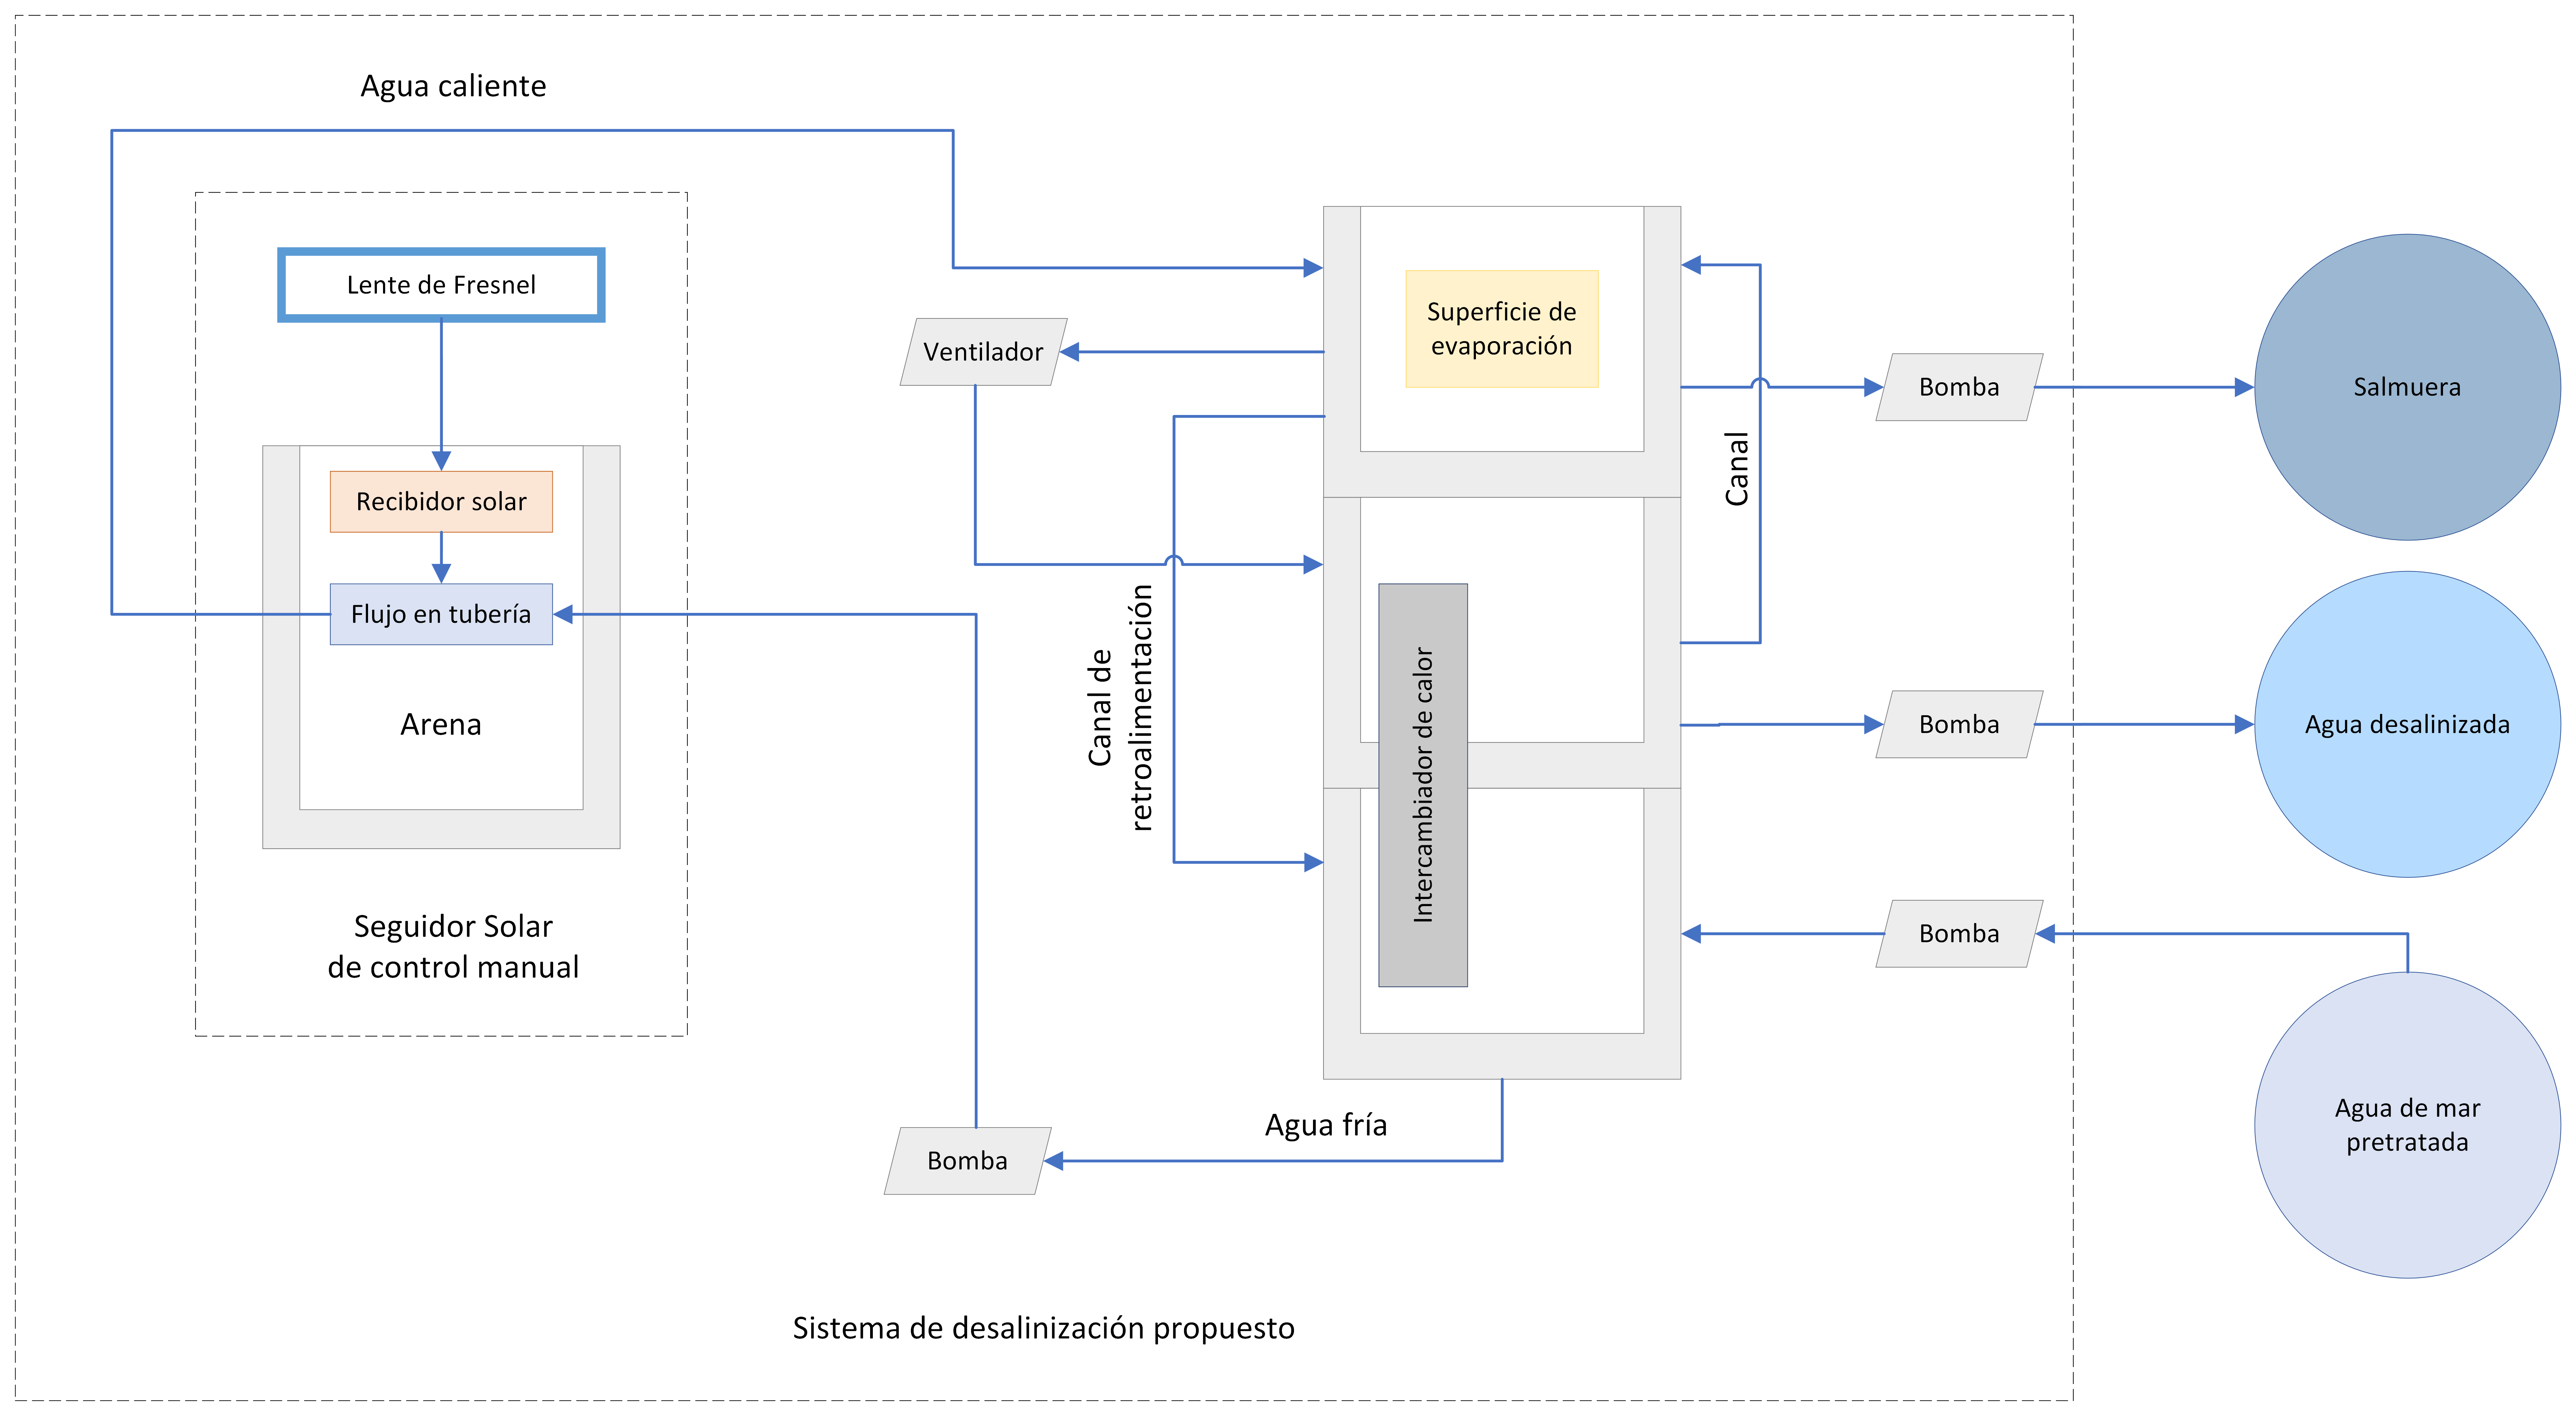
\includegraphics[
			    	width=\linewidth,
			    	height = 60mm,
			    	keepaspectratio
			]{Resultados/Sistema/VistaGeneral.png}
			\caption{Diagrama de funcionamiento del desalinizador}
	    \end{figure}		
	\end{frame}
	
	\begin{frame}
		\frametitle{Módulo de reaprovechamiento térmico y bombeo}
		\vspace*{2mm}
		
		\begin{figure}
		    	\centering
		    	\only<1>{
		    	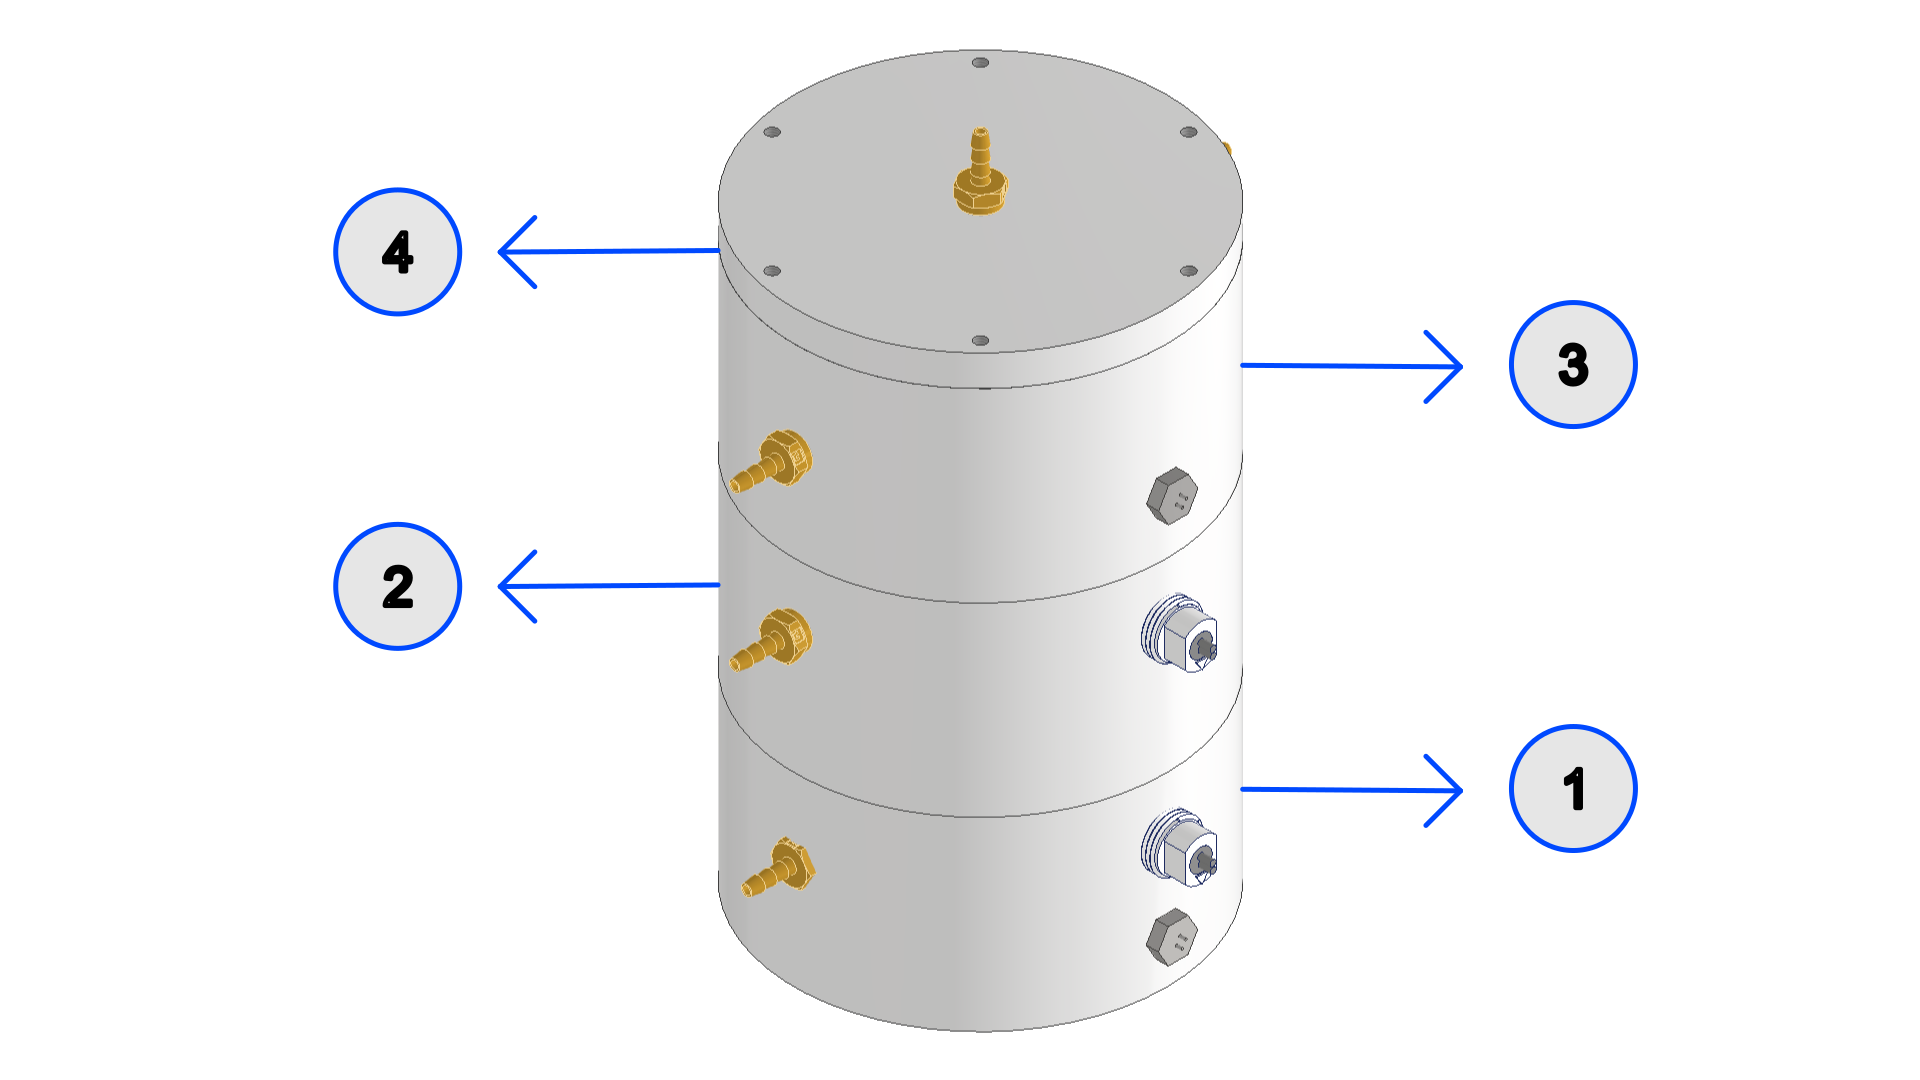
\includegraphics[
			    	width=\linewidth,
			    	height = 60mm,
			    	keepaspectratio
			]{Resultados/Sistema/WaterModule.png}
			\caption{Submódulos}
			}
			\only<2>{
		    	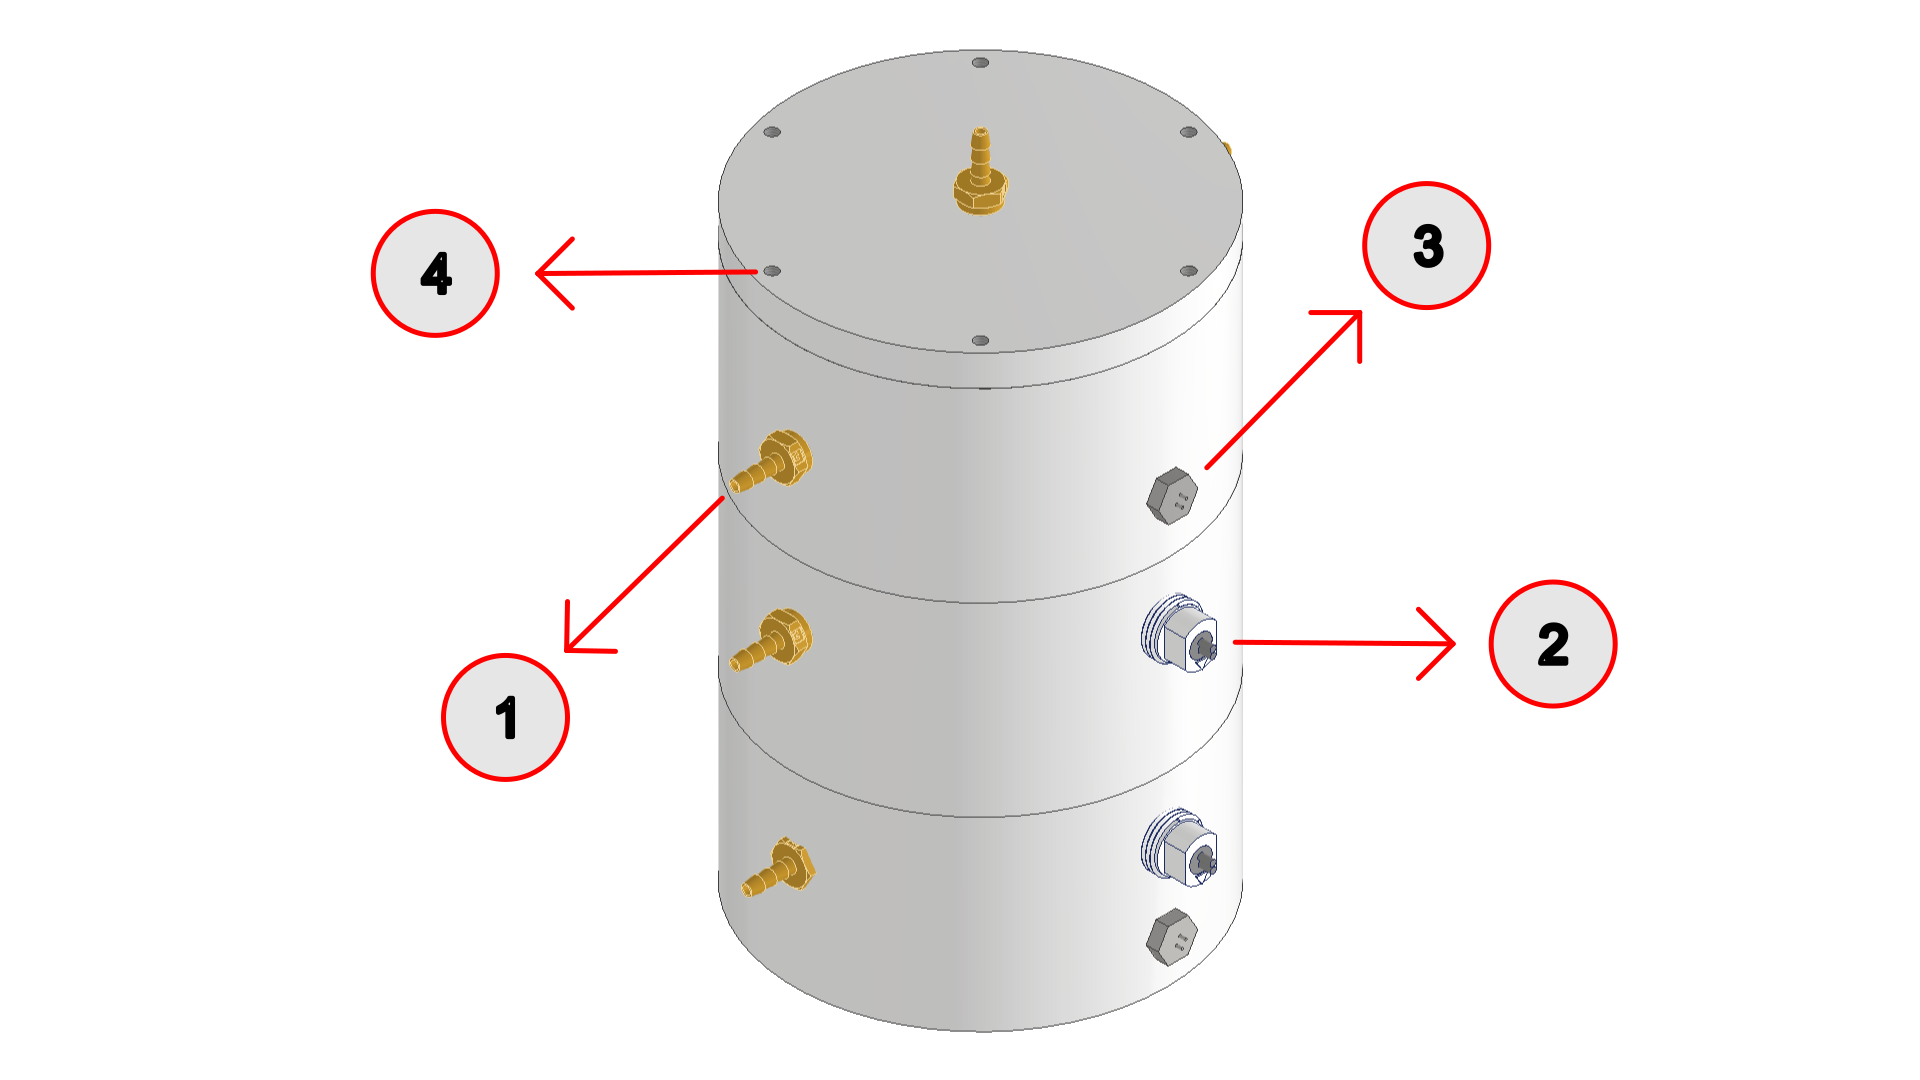
\includegraphics[
			    	width=\linewidth,
			    	height = 60mm,
			    	keepaspectratio
			]{Resultados/Sistema/WaterModuleComponents.png}
			\caption{Componentes}
			}
	    \end{figure}
	\end{frame}
	
	\begin{frame}
		\frametitle{Módulo de concentración solar}
		\vspace*{2mm}
		
		\begin{figure}
		    	\centering
		    	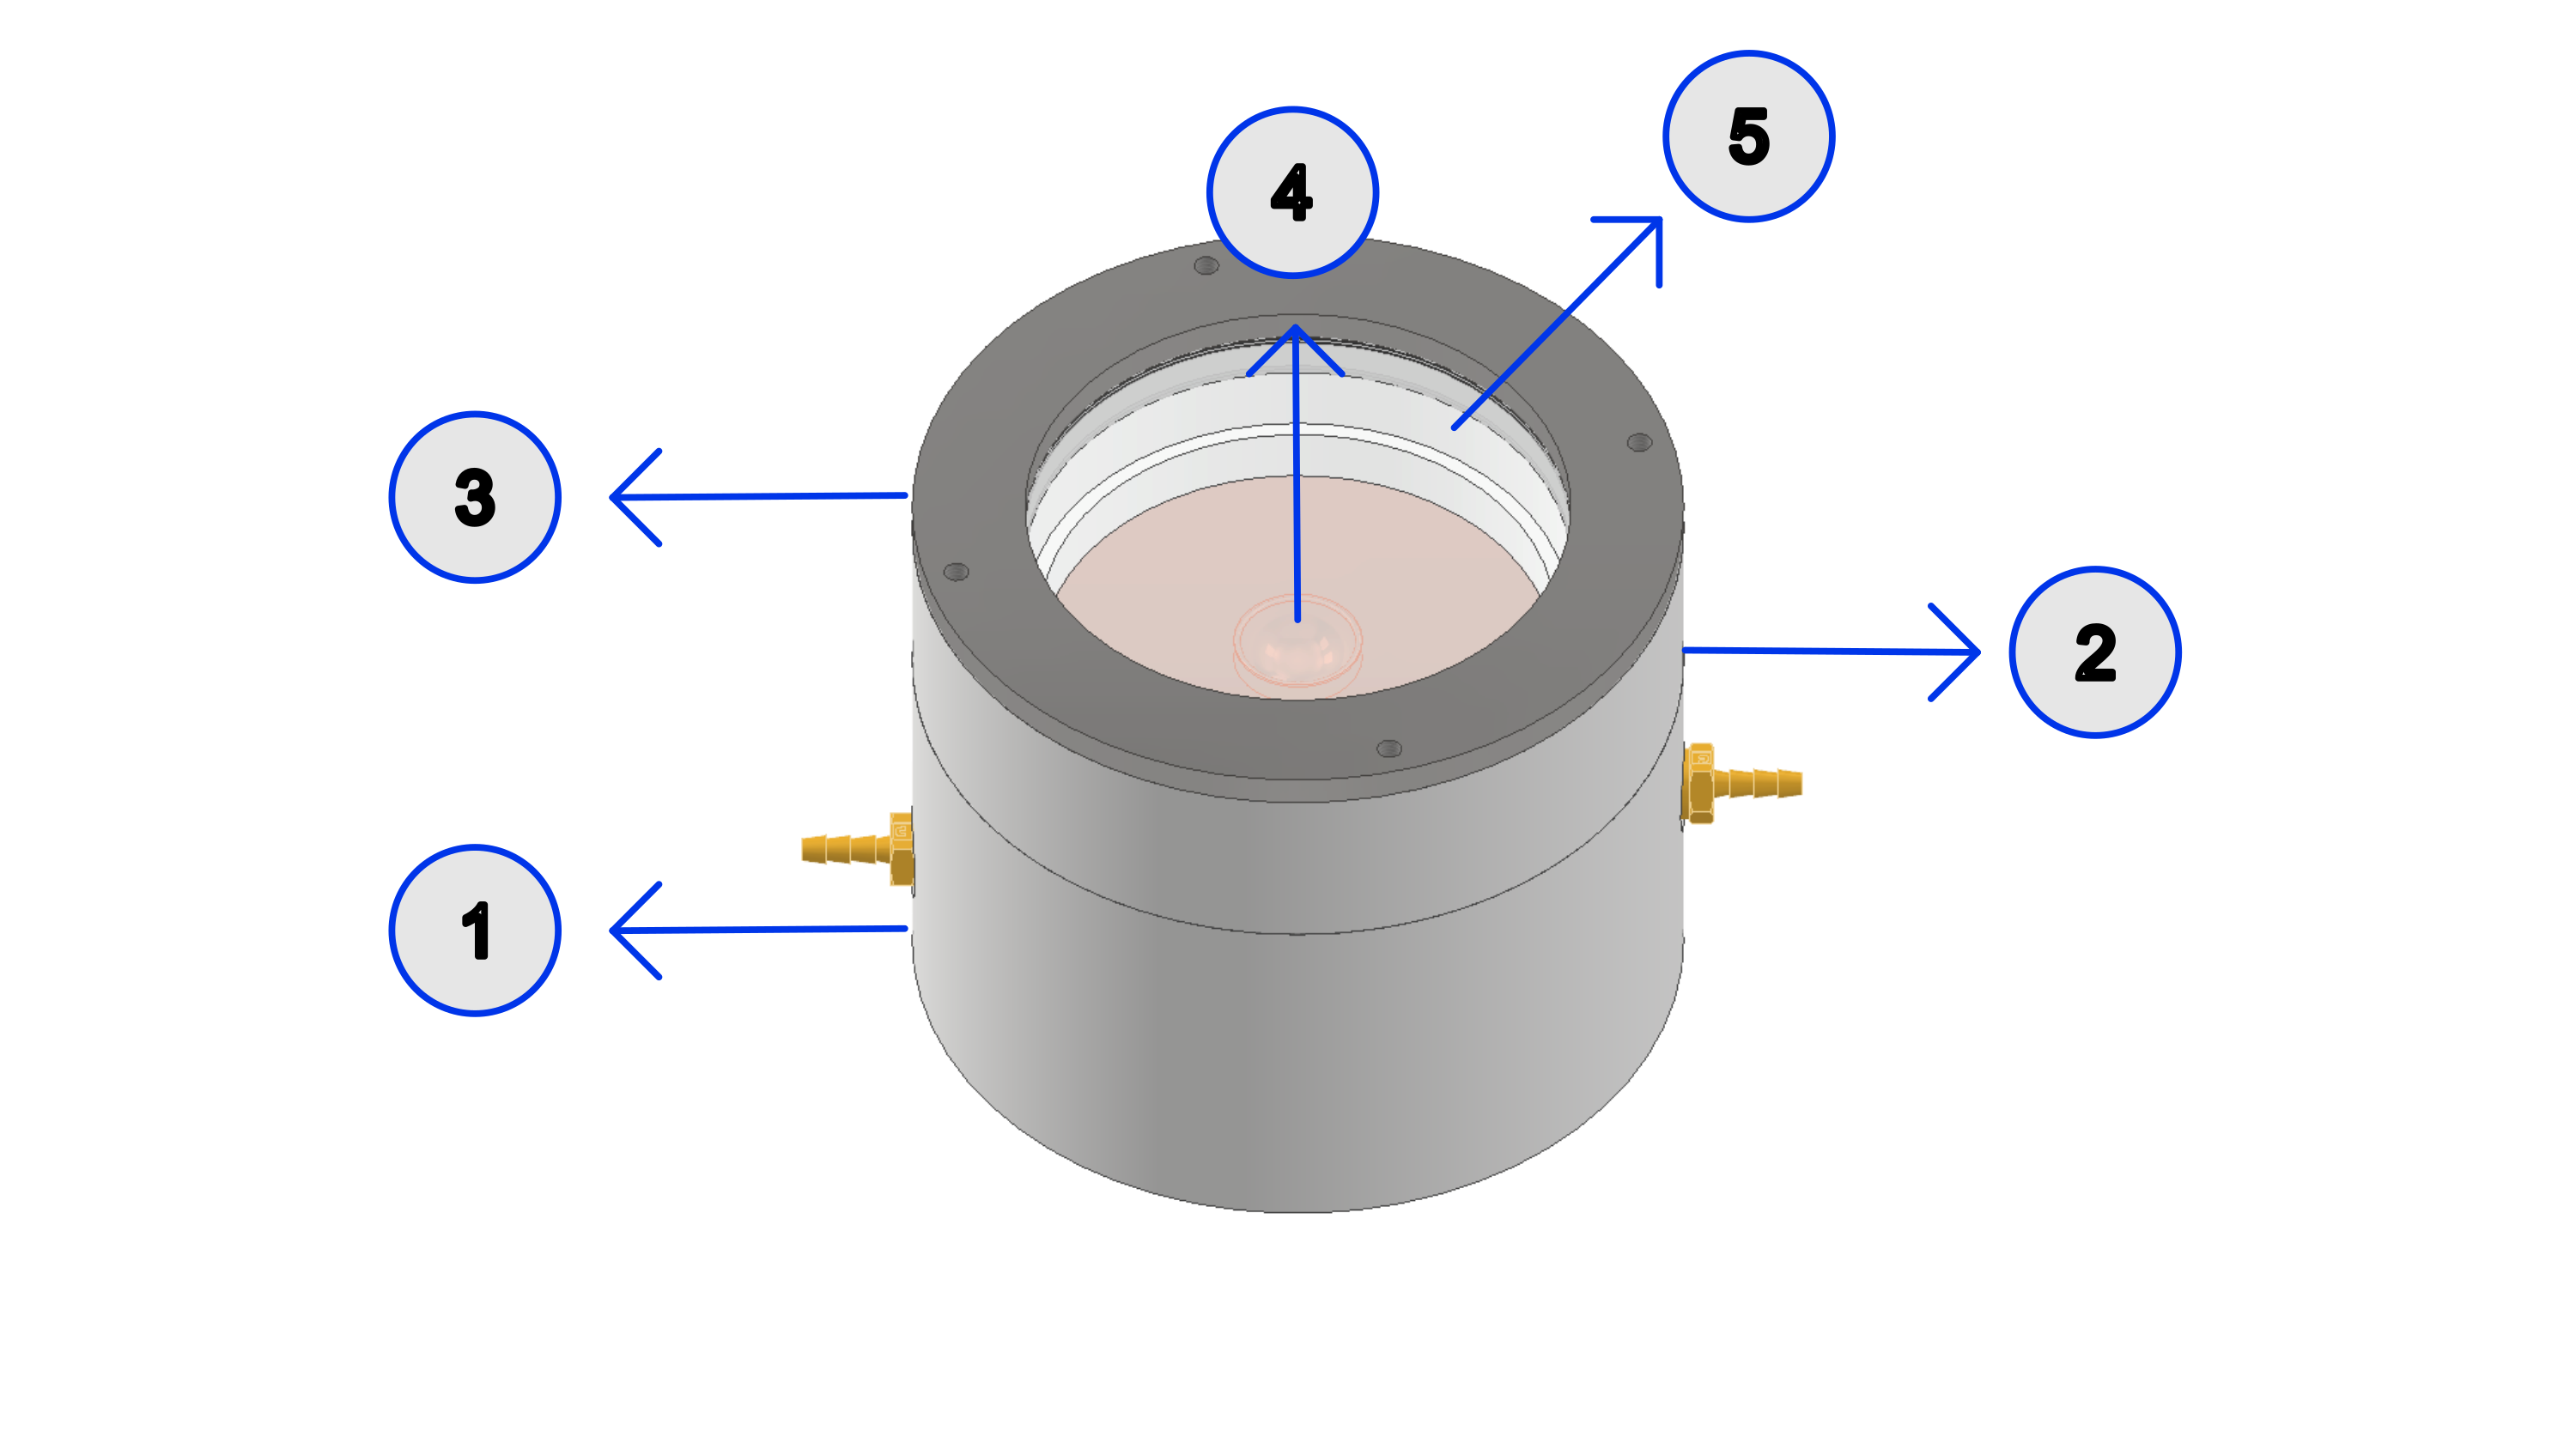
\includegraphics[
			    	width=\linewidth,
			    	height = 60mm,
			    	keepaspectratio
			]{Resultados/Sistema/SolarModule.png}
			\caption{Submódulos}
	    \end{figure}
	\end{frame}
	
	\begin{frame}
		\frametitle{Simulaciones}
		\vspace*{2mm}
		\begin{columns}
	    		\begin{column}{0.5\linewidth}
	    			\begin{figure}
	    				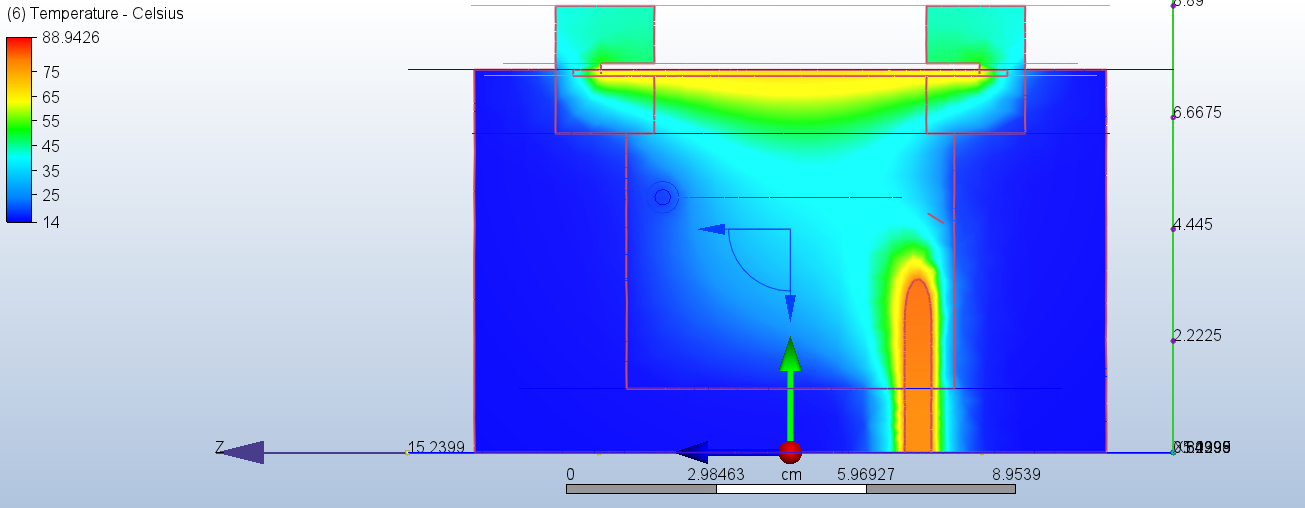
\includegraphics[
		    				width=\linewidth
	    				]{Resultados/Simulaciones/50WCopper15C9mlpm.png}
	    				\caption{Corte en la entrada y salida del agua de mar usando una tubería de cobre}
	    			\end{figure}
		    \end{column}
		    \begin{column}{0.5\linewidth}
		    		\begin{figure}
	    				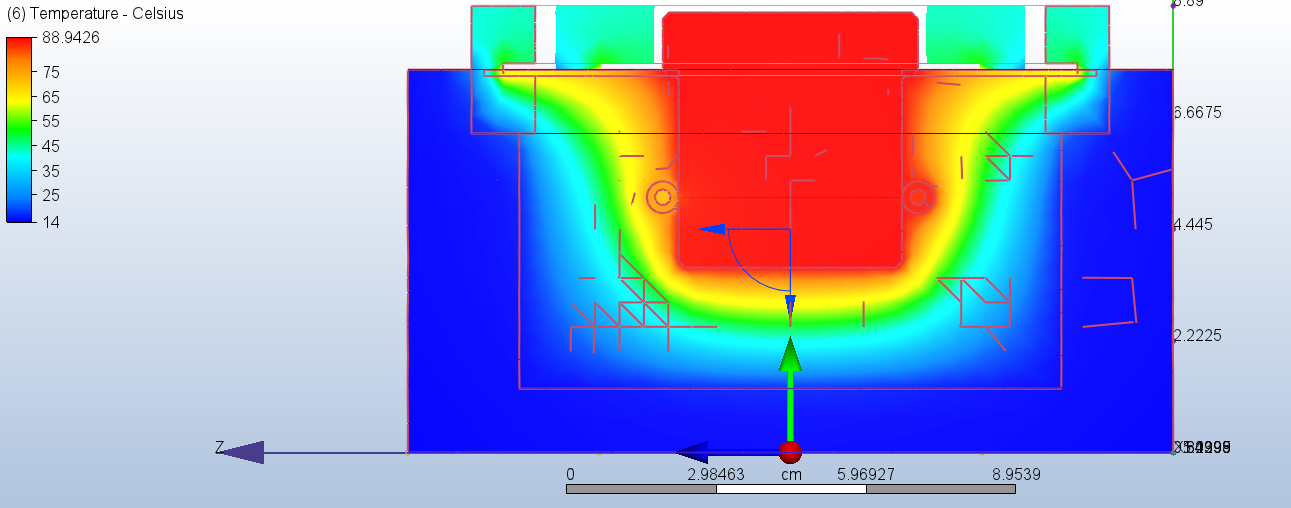
\includegraphics[
		    				width=\linewidth
	    				]{Resultados/Simulaciones/50WCopper15C9mlpm-middle.png}
	    				\caption{Corte en el centro del recibidor solar y su transferencia de calor hacia el cobre}
	    			\end{figure}
		    \end{column}
	    \end{columns}
	\end{frame}
	
	\begin{frame}
		\frametitle{Simulaciones}
		\vspace*{2mm}
		\begin{figure}
    			\includegraphics[
    				width=\linewidth,
    				height = 6cm,
    				keepaspectratio
    			]{Resultados/Simulaciones/FuzzyUniverse.png}
    			\caption{Simulaciones posteriores para determinar el universo de discurso del control difuso}
  		\end{figure}
	\end{frame}
	
	\begin{frame}
		\frametitle{Simulaciones}
		\vspace*{2mm}
		\begin{columns}
	    		\begin{column}{0.5\linewidth}
	    			\begin{figure}
	    				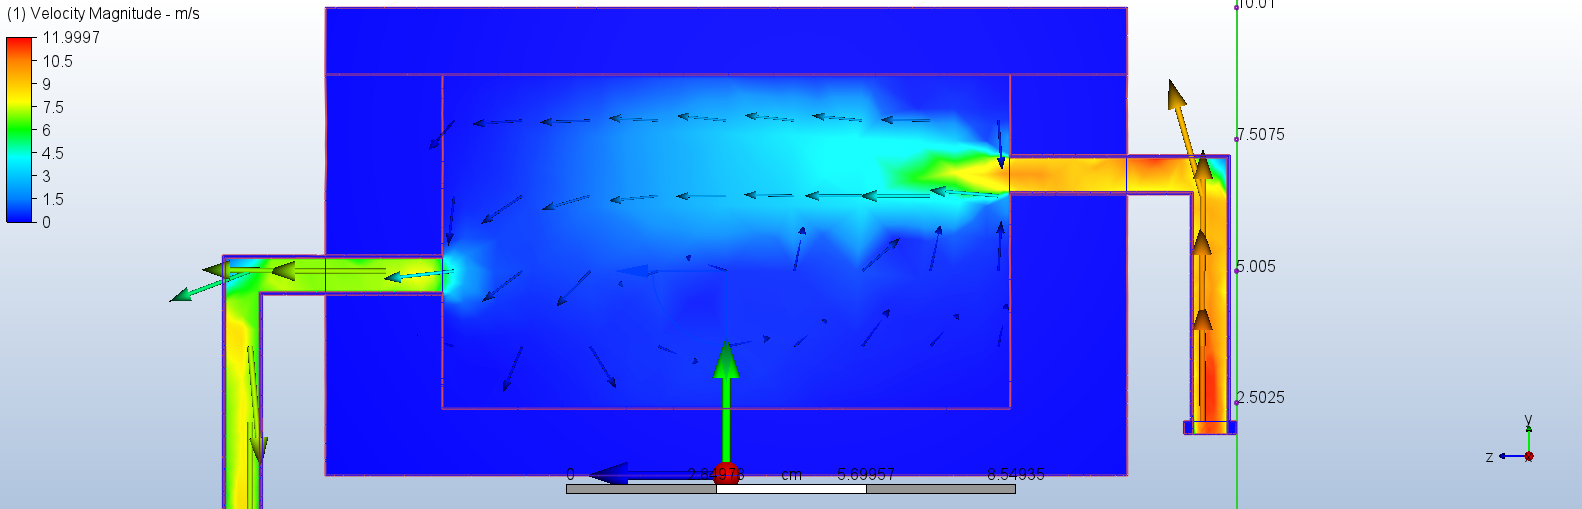
\includegraphics[
		    				width=\linewidth
	    				]{Resultados/Simulaciones/AirflowWithoutEvaporationSurface.png}
	    				\caption{Flujo de aire dentro de la cámara de evaporación sin la superficie de evaporación}
	    			\end{figure}
		    \end{column}
		    \begin{column}{0.5\linewidth}
		    		\begin{figure}
	    				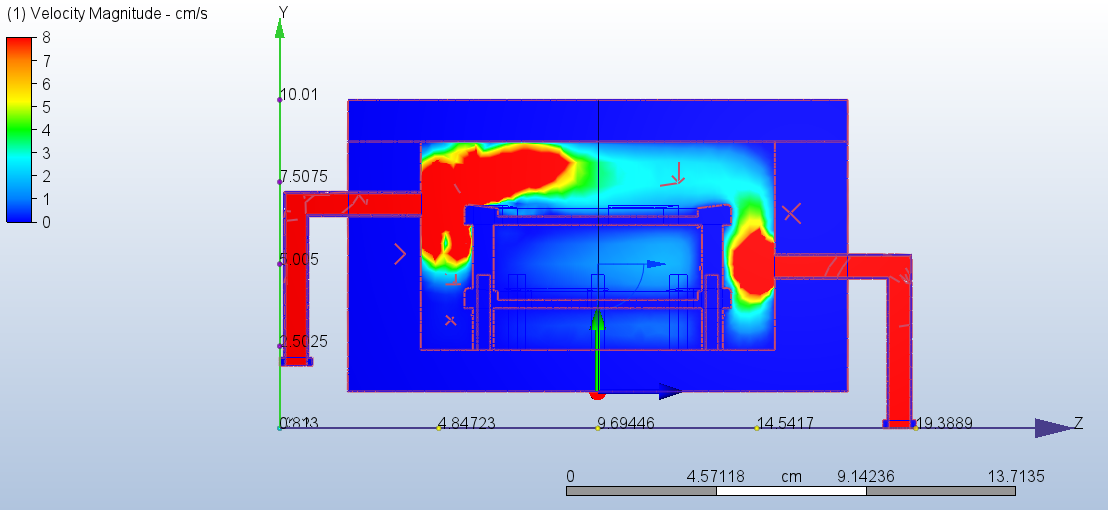
\includegraphics[
		    				width=\linewidth
	    				]{Resultados/Simulaciones/AirflowWithEvaporationSurface.png}
	    			\caption{Flujo de aire dentro de la cámara de evaporación con la superficie de evaporación}
	    			\end{figure}
		    \end{column}
	    \end{columns}		
	\end{frame}